\newpage
\section{Propuesta de Solución}
Para el desarrollo de este proyecto se utilizará la metodología VDI 2206, está basada en un enfoque concurrente (en lugar de secuencial), lo que resulta en productos con más sinergia. La integración sinérgica tiene como objetivo obtener mejores sistemas que la suma independiente de sus partes. Es posible optimizar los parámetros del diseño de cada fase del proceso de diseño con el fin de obtener la calidad y rendimiento deseados, consta de 3 elementos principales\cite{Referencia7}:
\begin{itemize}
    \item Solución de problemas a nivel micro.
    \item Modelo en V para el nivel macro.
    \item Definición de módulos para repetición de pasos durante el proceso de diseño mecatrónico.
\end{itemize}
\begin{center}
    \includegraphics[scale=0.55]{imagenes/Modelo en V.png}
    \captionof{figure}{Modelo en V \cite{Referencia7}}
    \label{fig:metodologia}
\end{center}
El punto inicio dentro del modelo en V es la \textbf{definición de requerimientos}, posteriormente se realiza un \textbf{diseño de sistema} con el objetivo de definir los conceptos de solución que describen las características físicas y lógicas del producto, las funcionalidades del sistema se dividen en subfunciones. A continuación se realiza el \textbf{diseño especifico por área del conocimiento}, donde se elabora el diseño y se realizan los cálculos necesarios para garantizar el desempeño particular de las funciones críticas. Después esta la \textbf{integración del sistema}, en este paso se integran los resultados del diseño específico para posteriormente ser analizados en la \textbf{validación y verificación}, considerando que las características del sistema cumplan con los conceptos de solución y los requerimientos. El producto resultante del macrociclo no necesariamente será el producto final ya que normalmente se requieren múltiples iteraciones para alcanzar cierto grado de madurez.\\
A continuación, se obtendrán los requerimientos y necesidades del proyecto, siguiendo con el desglose de las áreas funcionales y la propuesta de solución.
\subsection{Necesidades}
La metodología VDI 2206 emplea los requerimientos como entrada inicial del proceso, a continuación, se presentan las necesidades para después convertirlas en requerimientos.
\begin{itemize}
    \item Transporte de cobots rápido y preciso.
    \item Fácil instalación.
    \item Mantenimiento mínimo.
    \item Diferentes modos de operación (depuración y producción).
    \item Compatible con cobots de diferentes marcas.
    \item Control manual de movimiento.
    \item Controlable desde el ambiente de ROS.
    \item Seguridad para el operador humano.
    \item Parámetros de operación configurables.
    \item Operación por al menos 16 horas continuas.
    \item Fácil interfaz con operador humano.
    \item Comunicación con PC.
\end{itemize}
A partir del problema de diseño y enfoque del proyecto se plantea una clasificación de las necesidades del sistema, separándolas por áreas funcionales y no funcionales.

\begin{table}[ht]
\begin{center}
\begin{tabular}{|c|c|c|}
\hline
\multicolumn{3}{|c|}{\textbf{Necesidades por áreas funcionales}}                               \\ \hline
\textbf{ID} & \textbf{Necesidad}                                      & \textbf{Clasificación} \\ \hline
N1          & Transporte de cobots rápido y preciso.                  & Funcional              \\ \hline
N2          & Fácil instalación                                       & No funcional           \\ \hline
N3          & Mantenimiento mínimo                                    & No funcional           \\ \hline
N4          & Diferentes modos de operación (depuración y producción) & Funcional              \\ \hline
N5          & Compatible con cobots de diferentes marcas              & Funcional              \\ \hline
N6          & Control manual de movimiento                            & Funcional              \\ \hline
N7          & Controlable desde el ambiente de ROS                    & Funcional              \\ \hline
N8          & Seguridad para el operador humano                       & No funcional           \\ \hline
N9          & Parámetros de operación configurables                   & No funcional           \\ \hline
N10         & Operación por al menos 16 horas continuas               & No funcional           \\ \hline
N11         & Fácil interfaz con operador humano                      & Funcional              \\ \hline
N12         & Comunicación con PC                                     & No funcional            \\ \hline
\end{tabular}
\caption{Desglose de necesidades por áreas funcionales.}
\label{tab:cuadro_af}
\end{center}
\end{table}
\newpage
\subsection{Requerimientos}
Se procede a transformar las necesidades en requerimientos que permiten especificar el área funcional identificando los rangos de trabajo de cada uno de ellos. 

\begin{table}[ht]
\begin{center}
\begin{tabular}{|c|c|c|}
\hline
\multicolumn{3}{|c|}{\textbf{Requerimientos de Sistema}}                                                                                                         \\ \hline
\textbf{General} & \textbf{Específicos}                                               & \textbf{Rangos}                                                          \\ \hline
Geometría        & Longitud de carrera                                                & 400mm                                                      \\ \hline
Instalación      & Modo de instalación                                                & Sobre perfiles de aluminio                                               \\ \hline
Energía          & \begin{tabular}[c]{@{}c@{}}Temperatura\\ Alimentación\end{tabular} & \begin{tabular}[c]{@{}c@{}}10°C a 30°C\\ De línea a 127 Vca\end{tabular} \\ \hline
\end{tabular}
\caption{Rquerimientos detallados del sistema.}
\label{tab:cuadro_rs}
\end{center}
\end{table}


\begin{table}[ht]
\begin{center}
\begin{tabular}{|c|c|c|}
\hline
\multicolumn{3}{|c|}{\textbf{Requerimientos de Funcionalidad}}                                                                                                                                                                                                                                                   \\ \hline
\textbf{General} & \textbf{Específicos}                                                         & \textbf{Rangos}                                                                                                                                                                                                \\ \hline
Fuerza           & Capacidad de carga                                                           & \textgreater{}20Kg                                                                                                                                                                                             \\ \hline
Movimiento       & \begin{tabular}[c]{@{}c@{}}Posición\\ Velocidad\\ Repitibilidad\end{tabular} & \begin{tabular}[c]{@{}c@{}}1 GDL\\ \textgreater{}1 m/s\\ \textless{}1 mm\end{tabular}                                                                                                                          \\ \hline
Compatibilidad   & Modelos de Cobots                                                            & \begin{tabular}[c]{@{}c@{}}Universal Robots: UR3\\ Franka Emika: Panda\\ Pilz GmbH \& Co. KG: PRBT6\\ Kinova: Jaco, Jaco2 y MICO\\ UFACTORY: xArm5, xArm6, xArm7\\ aubo: i3\end{tabular} \\ \hline
Software         & \begin{tabular}[c]{@{}c@{}}Versión de ROS\\ Sistema Operativo\end{tabular}   & \begin{tabular}[c]{@{}c@{}}ROS 2  Foxy Fitzroy\\ Ubuntu 20.04\end{tabular} \\ \hline
\end{tabular}
\caption{Rquerimientos de Funcionalidad detallada.}
\label{tab:cuadro_rf}
\end{center}
\end{table}

\begin{table}[ht]
\begin{center}
\begin{tabular}{|c|c|c|}
\hline
\multicolumn{3}{|c|}{\textbf{Requerimientos de Usuario}}                                                                                                                                                                       \\ \hline
\textbf{General}                                              & \textbf{Específicos}                                                       & \textbf{Rangos}                                                                   \\ \hline
\begin{tabular}[c]{@{}c@{}}Modos de \\ operación\end{tabular} & \begin{tabular}[c]{@{}c@{}}Manual\\ Depuración\\ Producción\end{tabular}   & \begin{tabular}[c]{@{}c@{}}Uso de botones\\ Uso de botones y PC\\ PC\end{tabular} \\ \hline
Interfaz                                                      & \begin{tabular}[c]{@{}c@{}}Comunicación\\ Control\\ Monitoreo\end{tabular} & \begin{tabular}[c]{@{}c@{}}Protocolo RS-485\\ Botones\\ Pantalla\end{tabular}     \\ \hline
\end{tabular}
\caption{Rquerimientos de Usuario.}
\label{tab:cuadro_ru}
\end{center}
\end{table}
\newpage
\subsection{Diagramas funcionales}
Para desarrollar el diseño del sistema es necesario definir la función principal, así como las funciones y subfunciones, que desempeñará acorde a los requerimientos. A continuación, se plantean las funciones del sistema y se describe las características que permitirán asociar la información a los retos de diseño y precisar la complejidad del sistema.\\
\\
Función principal: \textbf{Movimiento}
\begin{enumerate}
    \item Gestión de Energía
    \begin{enumerate}[label*=\arabic*.]
        \item Monitoreo de suministro de energía eléctrica
        \item Subministrar energía
    \end{enumerate}
    \item Gestión de Información
        \begin{enumerate}[label*=\arabic*.]
        \item Procesamiento
            \begin{enumerate}[label*=\arabic*.]
            \item Control de posición
            \item Control de velocidad
            \item Recepción de instrucciones
            \item Retroalimentación de variables
            \item Sincronización con robot colaborativo
            \end{enumerate}
        \item Interfaz de Usuario
            \begin{enumerate}[label*=\arabic*.]
            \item Configuraciones del sistema
            \item Selección de modelo de robot colaborativo
            \item Selección de modo de operación
            \end{enumerate}
        \end{enumerate}
    \item Accionamiento mecánico
    \begin{enumerate}[label*=\arabic*.]
        \item Control manual
        \item Secuencia de calibración
        \item Ejecución de desplazamiento
        \item Mantenimiento y seguridad
        \begin{enumerate}[label*=\arabic*.]
            \item Detectar fin de carrera
            \item Detectar errores y accidentes
            \item Paro de emergencia
        \end{enumerate}
     \end{enumerate}
\end{enumerate}
La definición de Integración para el Modelado de Funciones (IDEF) es un proceso que permite una representación gráfica cualitativa. Presenta diferentes niveles de abstracción, tiene una semántica y sintaxis estandarizados y enriquecidos. Presenta el comportamiento estático del sistema y la interacción de los elementos funcionales y físicos. 
En la \textit{figura \ref{fig:idef_a0}} se muestra el nodo principal A0 con sus respectivas entradas y los productos de salida del sistema  que en este caso los más relevantes serían el movimiento sincronizado tanto del robot como del eje lineal. El nodo A0 se compone de otras 2 áreas o nodos, como se mencionó anteriormente y como se muestra en la\textit{ figura \ref{fig:idef_a0_expand}}, aquí también se puede observar las conexiones entre nodos que componen el sistema, un detalle relevante es la conexión directa de los controles manuales al nodo A3 y no a través del nodo A2, la razón es que se busca cierta independencia del nodo A2 en caso de una falla en el mismo o para facilitar la detección de errores durante el desarrollo del proyecto y la operación.

\begin{center}
    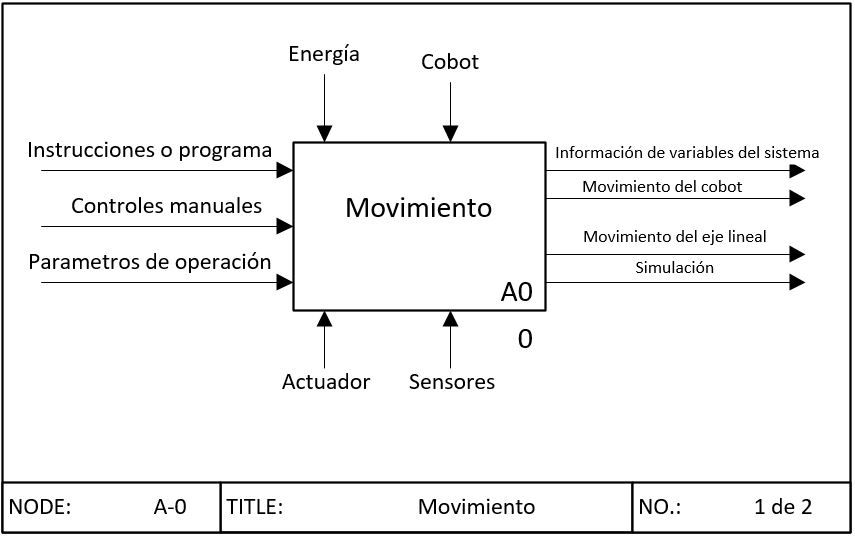
\includegraphics[scale=0.55]{imagenes/IDEF0_Protocolo_A-0.png}
    \captionof{figure}{Diagrama IDEF0}
    \label{fig:idef_a0}
\end{center}
\begin{center}
    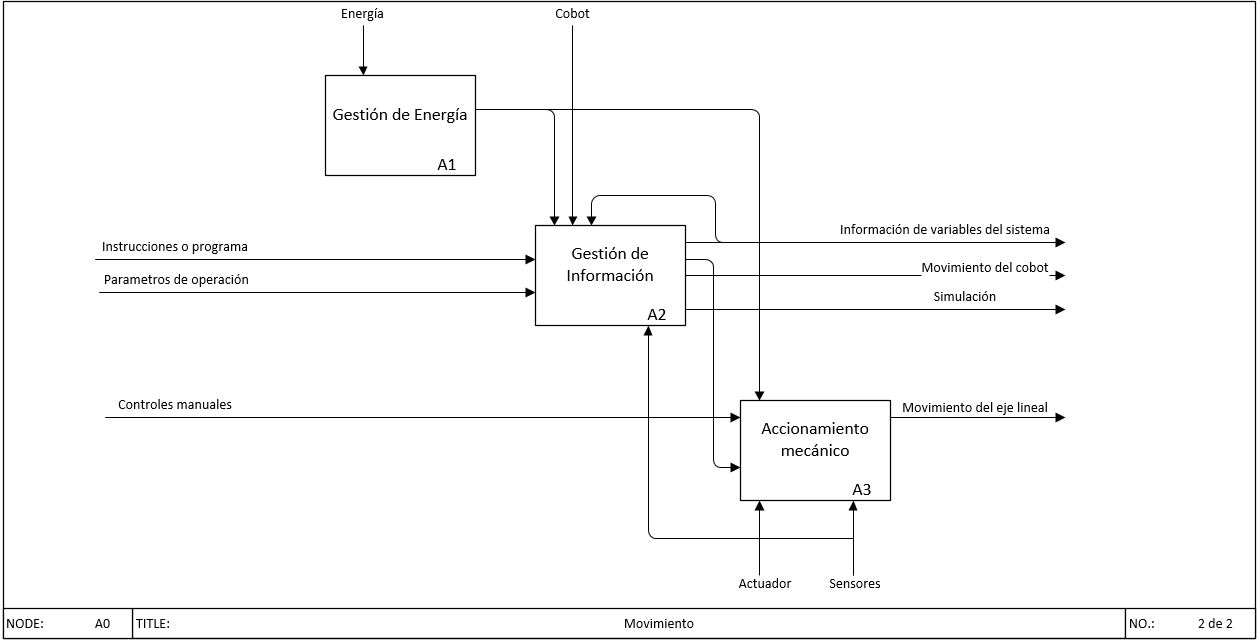
\includegraphics[scale=0.55]{imagenes/IDEF0_Protocolo_A-0_expandido.png}
    \captionof{figure}{Diagrama IDEF0 expandido}
    \label{fig:idef_a0_expand}
\end{center}

\subsection{Arquitectura física}
Utilizando las mismas áreas funcionales se establece a continuación los componentes físicos que se requerirán para el desarrollo del proyecto y de los cuales su arquitectura y particularidades se generaran durante la fase de diseño detallado.
\begin{enumerate}
    \item Gestión de Energía
    \begin{enumerate}[label*=\arabic*.]
        \item Fuente de alimentación fija.
    \end{enumerate}
    \item Gestión de Información
        \begin{enumerate}[label*=\arabic*.]
        \item CPU
        \item Microcontrolador
        \item Pantalla táctil
        \end{enumerate}
    \item Accionamiento mecánico
    \begin{enumerate}[label*=\arabic*.]
        \item Estructura
        \item Guía lineal
        \item Interfaz de botones
        \item Microcontrolador
        \item Servomotor
        \item Sensores
     \end{enumerate}
\end{enumerate}
\begin{center}
    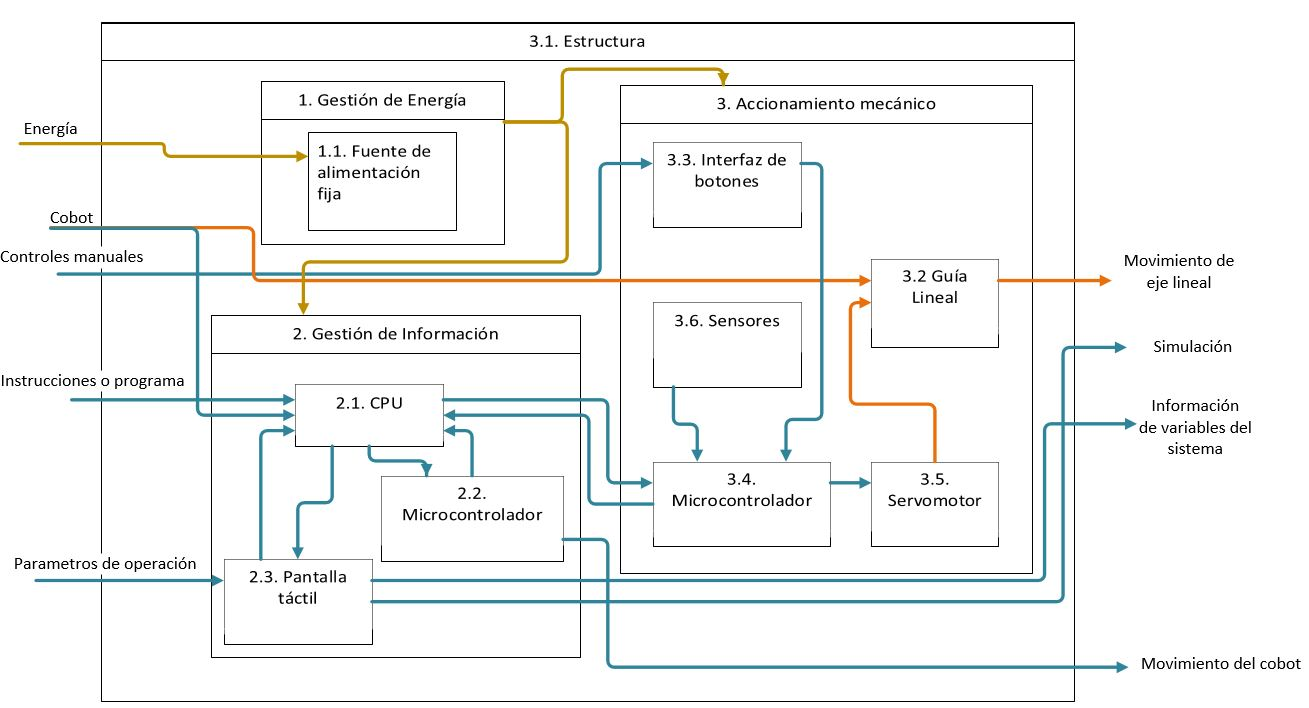
\includegraphics[scale=0.45]{imagenes/Arquitectura del TT.JPG}
    \captionof{figure}{Diagrama de la arquitectura física}
    \label{fig:idef_af}
\end{center}
\subsection{Resultados esperados}
Con lo anteriormente mostrado se busca construir un séptimo grado de libertad de tipo prismático para robots colaborativos de menor de 20kg de peso (incluyendo la capacidad de carga del robot), todos los elementos del proyecto estarán embebidos en una misma estructura, la cual será de fácil instalación sobre estructuras hechas con perfiles de aluminio. El sistema tendrá una pantalla táctil que mostrará la interfaz gráfica del sistema operativo y donde se pondrán a ejecutar comandos y programas para el robot, dentro de esta interfaz se podrá visualizar y modificar los parámetros de funcionamiento del robot, así como al modo de operación.\\
Para lograr la compatibilidad con los modelos mencionados en la \textit{tabla \ref{tab:cuadro_rf}} se diseñara una base intercambiable para cada modelo de robot, además se diseñara y construiría toda la interfaz necesaria para controlar los robots aunque es importante señalar que no se probara el funcionamiento del eje lineal con alguno de los modelos debido al elevado costo de estos, en lugar de esto se realizara una simulación en tiempo real en un ambiente 3D de ROS donde se aprecie el movimiento del robot colaborativo y el movimiento del proyecto; mientras que de manera física se observara el desplazamiento del eje lineal. Para estas demostraciones se programará el robot con trayectorias de prueba que se encuentren fuera del área de trabajo de fábrica, el robot debe seguir las trayectorias utilizando el eje lineal como si fuera un grado de libertad adicional. En el modelo físico se colocarán pesos de prueba que representen el de un robot colaborativo, el eje lineal deberá moverse de acuerdo con los parámetros que el usuario haya seleccionado y a la trayectoria que se le haya programado o alternativamente usando los controles manuales.\\
Uno de los propósitos de este proyecto es ampliar las posibilidades del software libre y de código abierto en el mundo de la robótica por ello el producto final contara con su propia paquetería de ROS que estará disponible para cualquier persona pueda usarla, modificarla o contribuir mejoras. Este paquete de software se usará para conectar el hardware del robot al ambiente ROS por lo que no solo servirá para sincronizarse con módulos de planeación de trayectorias si no que se podrá conectar con todos las herramientas y módulos disponibles en ROS, otorgando flexibilidad en el diseño de sistemas robóticos para el usuario final.\\

